
%   i.) Describe all the steps of a Deep Learning FL system
%      
%

%how do FL systems work in general?
Feature location systems retrieve a ranked list of program elements
(e.g. methods, classes) for a developer query. In the {\em indexing}
phase, feature location systems commonly construct a model of the
software, at the granularity of program elements, based on the natural
language embedded in identifiers and comments. In the {\em retrieval}
phase, given a natural language query, feature location systems use
the model to retrieve all of the relevant program elements with high
similarity to the query.

\subsection{Feature Location Workflow}

%how does a deep learning system differ
A feature location system based on deep learning, during its indexing
phase, creates a contextual representation of the natural language
terms embedded in the source code. This contextual representation
includes influence from terms preceding and following each term,
relative to their distance from that term. More intuitively, such
models incorporate mutual influence between terms in the same method,
while terms that are closer in distance (e.g. occur the same
statement) influence each other more strongly. 



\begin{figure}[tb]
\centering
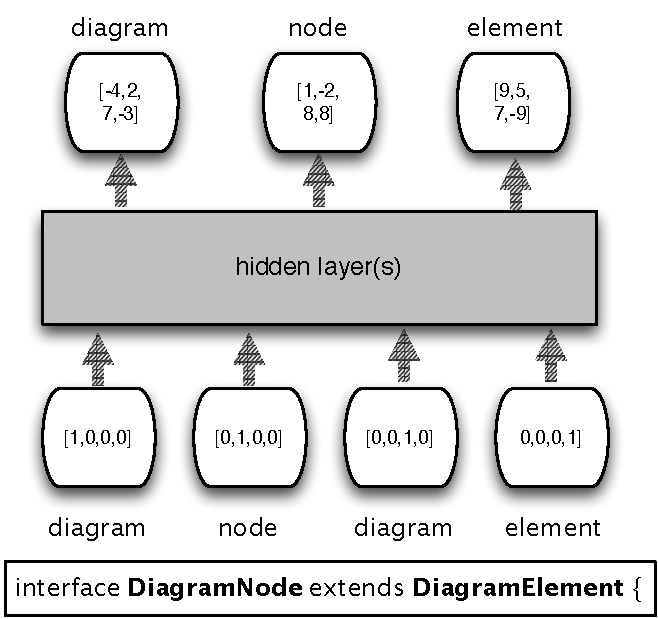
\includegraphics[width=.9\columnwidth]{figures/neuralnet.pdf}
\caption{A deep learning neural network encodes source code identifiers,
in the order they appear in the source code, in its input
layer. Using a deep structure of hidden layers, each term and its
context receives a semantic vector representation.}
\label{fig:neuralnet}
\end{figure}



%what is deep learning
Deep learning is based on a multi-stage neural network, consisting of
several hidden layers in addition to single input and output layers.
The input layer consists of an ordered sequences of identifiers
extracted from the code. The multiple hidden layers serve to capture
the context for each encountered term, representing the complex
patterns of term contexts occurring in the corpus. The output layer
consists of a vector for each term, which has been shown to carry
semantic meaning. An example of this architecture for a single line of
code is shown in Figure~\ref{fig:neuralnet}. Recent advances in this
area have stemmed from the use of novel neural network architectures,
including recurrent neural networks that connect the hidden layers
back to the input layer, among other strategies. The systems are
trained using backpropagation and gradient descent, techniques common
to many neural network based models.

 
%preprocessing
A number of preprocessing steps are commonly performed during the
indexing phase of feature location systems including word stemming,
which reduces terms to their base form (e.g. running $\rightarrow$
run), and stop word removal, which removes common words (e.g. the, is,
at). Additional preprocessing steps are required for source code, such
as identifier splitting, ensuring that composite identifiers are
divided into their constituent terms (e.g. addToCart $\rightarrow$
add,to,cart). 


During the retrieval state of feature location, a similarity measure
(e.g. cosine similarity) between the words in the query and words in
each program element is computed. The program elements are ranked
based on this similarity metric and presented to the developer in
descending order.

%Chris: we can talk about inference here too, not sure what you have planned

\subsection{Semantic Similarity}

The result of the deep learning models described in this paper are
vectors representing each term in the
corpus~\cite{mikolov_distributed_2013}. Similar vectors can also be
computed to represent an entire paragraph or
document~\cite{le_distributed_2014}.  Semantic similarity is the
notion that these vector are composable semantically (e.g. the result
of the operation {\em vec(``Montreal Canadians'') - vec(``Montreal'') +
vec(``Toronto'')} is closest to {\em vec(``Toronto Maple Leafs'')}). This
capability is established automatically by the system, without any
additional processing or labeled input.

In feature location, as in general information retrieval, the
retrieval quality can only be as good as the quality of the developer
query. Problems such as the dictionary mismatch problem, as well as
the propensity of users to issue short queries, have previously been
observed as common difficulties in feature
location~\cite{haiduc_effect_2011, damevski_field_2015}. Semantic
similarity can be a useful capability in mitigating these problems, by
performing query recommendation and automatic query extension.

To illustrate this capability for source code based corpora, we
provide a set of illustrative examples gathered on the ArgoUML project
(v. 0.22) (\url{http://argouml.tigris.org}) in Table~\ref{tab:semsim}.


\begin{table}[h!]
\centering
\small
\caption{Examples of semantically similar terms and their weight for a deep model trained on
the ArgoUML code base. Only terms with weight > 0.6 are included.}
\label{tab:semsim}
\begin{tabular}{|p{0.20\columnwidth}|p{0.70\columnwidth}|}
\hline \hline
Term(s) & Semantically Similar Terms and Weight\\ \hline 
association & (roles 0.75), (role 0.72), (classifier 0.72), ('connection', 0.61) \\ \hline
save & (saved 0.69), (pcs 0.64), (exists 0.63), (projects 0.60), (close, 0.61), (file 0.60) \\ \hline
file & [filter 0.78), (zip 0.74), (exists 0.74), (persister 0.71), (files 0.69), (directory 0.69) \\ \hline
explorer, option, creating, diagrams, elements, useful, lost, diagram, particular & (makes 0.68), (unwanted 0.68), (design 0.67), (commented 0.67) \\
\hline \hline
\end{tabular}
\end{table}

